\documentclass[11pt,a4paper]{article}
\usepackage[utf8]{inputenc}
\usepackage[T1]{fontenc}
\usepackage[spanish]{babel}
\usepackage[margin=2.5cm]{geometry}
\usepackage{graphicx}
\usepackage{longtable}
\usepackage{booktabs}
\usepackage{array}
\usepackage{xcolor}
\usepackage{colortbl}
\usepackage{hyperref}
\usepackage{enumitem}
\usepackage{fancyhdr}
\usepackage{titlesec}
\usepackage{caption}
\usepackage{tabularx}

\hypersetup{colorlinks=true,linkcolor=blue,urlcolor=blue,citecolor=blue}
\definecolor{uteqgreen}{RGB}{27,94,32}

\titleformat{\section}{\large\bfseries\color{uteqgreen}}{\thesection}{0.6em}{}
\titleformat{\subsection}{\normalsize\bfseries}{\thesubsection}{0.6em}{}

\pagestyle{fancy}
\fancyhf{}
\rhead{PE4 -- Unidad IV -- Equipo AHMRV}
\lhead{Ingeniería de Requisitos (ISR-401)}
\rfoot{\thepage}

\newcolumntype{Y}{>{\raggedright\arraybackslash}X}

\title{\vspace{-2cm}}
\date{}

\begin{document}

% ============================================================
% 1. CARÁTULA
% ============================================================

\begin{titlepage}
    \centering

    \textbf{\large UNIVERSIDAD TÉCNICA ESTATAL DE QUEVEDO}\\[0.5cm]

    
\includegraphics[width=4cm]{logo.png}\\[0.5cm]

    \textbf{INGENIERÍA DE REQUERIMIENTOS}\\[0.5cm]

\textbf{Link del Github}\\[0.5cm]

\url{https://github.com/equinteroj/ISR401-PFC-ERS-EQUIPO-I.git}

    \textbf{TEMA:}\\[0.3cm]

   VALIDACIÓN, GESTIÓN DE REQUISITOS Y HERRAMIENTAS CASE.\\[0.5cm]

    \textbf{INTEGRANTES:}\\[0.5cm]
   ESCUDERO PLAZA MARIA DEL ROSARIO\\[0.3cm]
    HUILCAPI LEON DENISSES FABIOLA\\[0.3cm]
    QUINTERO GENDE ERICK JAHIR\\[0.3cm]


    \textbf{ASIGNATURA:}\\[0.3cm]

    INGENIERÍA DE REQUERIMIENTOS\\[0.3cm]

    \textbf{CURSO:}\\[0.3cm]

    4TO “A” SOFTWARE\\[0.3cm]

    \textbf{FECHA:}\\[0.3cm]

    04/08/2026\\[0.3cm]

    \textbf{DOCENTE:}\\[0.3cm]

    ING. GUERRERO ULLOA GLEISTON CICERON\\[0.5cm]

 ULTIMO COMMIT FECHA MIERCOLES 5 DE JULIO 23:00 PM

    \vfill



\end{titlepage}

% ============================================================
% 2. RESUMEN Y OBJETIVOS
% ============================================================
\section{Resumen y objetivos}

Este informe documenta la Práctica Experimental de la Unidad IV aplicada sobre el ERS/SRS del
sistema SIMPA (Entrega 3, 2A, v3.0). El equipo ejecutó una inspección formal tipo Fagan que
consolidó 16 defectos únicos (3 críticos, 8 mayores, 5 menores) sobre una densidad de 0,40
defectos por página; corrigió el 100\,\% de los defectos críticos y mayores; tramitó tres
solicitudes de cambio (alcance, calidad y restricción normativa) ante un Change Control Board
simulado que produjo la versión v3.1 del ERS; construyó la trazabilidad bidireccional del
documento en un tablero Jira con cinco épicas, veinte historias y campos personalizados de
prioridad MoSCoW y fuente de evidencia; publicó la línea base \texttt{baseline-v3.1} en un
repositorio Git con historial semántico distribuido; y cerró con una comparativa de herramientas
CASE y una discusión contrastada entre la Ingeniería de Requisitos (IR) documental y la ágil.

\textbf{Objetivo general.} Aplicar técnicas formales de validación de requisitos, gestionar
cambios mediante un Change Control Board simulado, implementar la trazabilidad del ERS en una
herramienta CASE, establecer una línea base con Git y comparar metodológicamente la IR
tradicional frente a la IR ágil, sobre el ERS real del sistema SIMPA.

\textbf{Objetivos específicos.} (1) Ejecutar la inspección Fagan con roles diferenciados y
registro de defectos; (2) calcular e interpretar métricas de inspección; (3) tramitar tres RFC
con análisis de impacto sustentado en la matriz de trazabilidad; (4) deliberar y decidir en un
CCB simulado; (5) construir la trazabilidad bidireccional en Jira; (6) publicar la línea base con
Git; (7) comparar herramientas CASE y contrastar IR tradicional frente a IR ágil.

% ============================================================
% 3. FUNDAMENTO TEÓRICO
% ============================================================
\section{Fundamento teórico}

\subsection{Marco normativo}

La validación de requisitos se ubica formalmente en la cláusula 6.4 de
ISO/IEC/IEEE 29148:2018, que la distingue del proceso de definición de requisitos al exigir
evidencia de que el conjunto especificado es correcto, completo y aceptable para las partes
interesadas antes de avanzar a diseño. El control de cambios, por su parte, corresponde a los
procesos de gestión de la configuración de ISO/IEC/IEEE 15288:2023 (ciclo de vida de sistemas) y
ISO/IEC/IEEE 12207:2017 (ciclo de vida de software), que exigen trazabilidad entre la solicitud
de cambio, su análisis de impacto y la nueva línea base resultante. El modelo de calidad de
producto de ISO/IEC 25010:2023 se emplea en este informe como criterio de fondo para clasificar
los defectos de inspección (adecuación funcional, fiabilidad, seguridad, mantenibilidad,
compatibilidad, entre otras características ya cuantificadas en el ERS base). La guía
SWEBOK v4.0, en sus áreas 1.6--1.8, describe la validación, la gestión de requisitos y las
herramientas de soporte como procesos continuos y no como hitos aislados, postura que este
informe sigue al tratar la inspección, el CCB y la trazabilidad como un ciclo retroalimentado y
no como pasos secuenciales independientes. El Change Control Board, como cuerpo de decisión
formal sobre solicitudes de cambio con autoridad para aprobar, rechazar o diferir, se define
conforme al PMBOK 7.\textsuperscript{a} ed. como parte del proceso de control integrado de
cambios, y su composición multi-rol (cliente, analista, desarrollador, presidente) es la que se
reproduce en la simulación de la sección 6.

\subsection{Validación de requisitos}

La verificación responde a la pregunta \emph{¿se construyó el producto correctamente?} y se
apoya en criterios internos de consistencia; la validación responde a \emph{¿se construyó el
producto correcto?} y exige el contraste con la necesidad real del interesado. Entre las técnicas
de validación disponibles ---revisión informal, walkthrough, inspección formal, prototipado y
listas de verificación--- la inspección formal tipo Fagan es la más costosa de ejecutar pero la
que exhibe mayor tasa de detección temprana de defectos, por su estructura de roles
diferenciados y su prohibición explícita de discutir soluciones durante la reunión de detección
\cite{yousaf2022}. El método original de Fagan comprende cuatro fases ---planificación,
preparación individual, reunión de inspección y corrección--- y su vigencia se sostiene en
estudios empíricos recientes que replican el procedimiento sobre documentos de especificación de
requisitos y reportan mejoras medibles en la tasa de detección de defectos y en la reducción de
costo de corrección tardía \cite{yousaf2022}. La calidad de los requisitos que la inspección
busca proteger se organiza, según la revisión sistemática de Montgomery et al., en torno a un
número reducido de atributos dominantes ---ambigüedad, completitud, consistencia y
corrección--- que concentran la mayoría de los estudios empíricos publicados en el campo
\cite{montgomery2022}, atributos que este informe adopta como columnas de clasificación del
registro de defectos (Anexo B). Un caso particular de verificabilidad que la inspección de este
informe debió tratar de forma diferenciada es el de los requisitos no funcionales de
explicabilidad de los componentes de inteligencia artificial del SIMPA (RNF-16), cuya
especificación debe ser evaluable mediante prueba de comprensión con usuarios reales y no
solamente mediante inspección documental, conforme al marco de calidad de la explicabilidad como
requisito no funcional \cite{chazette2020} y a su posterior operacionalización en un catálogo de
tipos de explicación y técnicas de verificación \cite{chazette2021,chazette2022}.

\subsection{Gestión de requisitos}

La gestión de requisitos comprende la gestión de la configuración del documento (versión,
historial de cambios, línea base), los atributos asociados a cada requisito (prioridad, fuente,
estado, esfuerzo) y la trazabilidad, entendida en dos sentidos: la trazabilidad hacia atrás
(pre-traceability), que vincula el requisito con su origen en la evidencia de elicitación, y la
trazabilidad hacia adelante (post-traceability), que lo vincula con los artefactos de diseño,
código y prueba que lo satisfacen \cite{wang2024}. La matriz de trazabilidad es el instrumento
que materializa ambos sentidos en una sola estructura tabular y es también el insumo obligatorio
del análisis de impacto de toda solicitud de cambio (RFC): sin recorrer la matriz, ese análisis
se reduce a una estimación no verificable. El proceso de cambio formal sigue cuatro pasos:
solicitud (RFC) con su justificación de negocio, análisis de impacto derivado de la matriz,
decisión del CCB con su acta motivada, e implementación con el cierre correspondiente en el
historial de versiones. La volatilidad de requisitos --el cociente entre requisitos modificados,
añadidos o eliminados y el total de requisitos vigentes en un período-- es la métrica que permite
distinguir un proceso de cambio saludable de uno errático; en este informe se reporta en la
sección~8 tras la implementación de las tres RFC.

\subsection{Herramientas CASE para IR}

Las herramientas de asistencia a la ingeniería de software (CASE) para requisitos se clasifican
en \emph{upper-CASE} (elicitación y modelado), \emph{lower-CASE} (generación de artefactos hacia
implementación) e \emph{integradas}, que cubren el ciclo completo. Para la gestión de requisitos
en particular, las funcionalidades esperables son: repositorio central del requisito con su
identificador estable, atributos personalizables, trazabilidad bidireccional visualizable,
mecanismo de línea base (baselining), flujo de control de cambios con estados, colaboración
multiusuario e integración con sistemas de control de versiones (VCS). Jira y Trello, empleadas
en este informe, son herramientas ágiles de gestión de flujo de trabajo que aproximan estas
funciones mediante Epics/Stories/Sub-tasks y campos personalizados, mientras que herramientas
especializadas en IR --como las comparadas en la sección~9-- ofrecen trazabilidad nativa
bidireccional y auditoría de cambios más robusta, a costa de una curva de aprendizaje y un costo
de licenciamiento mayores. La incorporación de procesamiento de lenguaje natural en estas
herramientas para detectar automáticamente vínculos de trazabilidad o defectos de redacción sigue
siendo, según la revisión sistemática de Zhao et al., un campo activo pero con baja adopción
industrial fuera de prototipos académicos \cite{zhao2021}, lo que en este informe se traduce en
que la trazabilidad de la sección~7 se construyó manualmente y no de forma asistida.

\subsection{IR en procesos ágiles}

En los procesos ágiles el requisito se expresa habitualmente como historia de usuario en formato
Connextra (\emph{Como \dots\ quiero \dots\ para \dots}), organizada en un \emph{product backlog}
priorizado y sometida a sesiones de \emph{grooming} que la descomponen hasta cumplir con una
\emph{Definition of Ready}. La revisión sistemática de Raharjana et al. sobre el uso de
procesamiento de lenguaje natural en historias de usuario documenta que la ambigüedad y la
heterogeneidad de formato siguen siendo el problema dominante de este artefacto, lo que justifica
la exigencia de criterios de aceptación formales \cite{raharjana2021}. El formato Gherkin
(\emph{Dado \dots\ Cuando \dots\ Entonces \dots}), propio del desarrollo guiado por
comportamiento (BDD), traduce cada criterio de aceptación en un escenario ejecutable que conecta
la historia de usuario con la prueba automatizada, cerrando así el ciclo de trazabilidad sin
recurrir a una matriz externa. Frente a la IR documental --que privilegia la especificación
completa antes de construir y una trazabilidad explícita y auditable-- la IR ágil privilegia la
retroalimentación iterativa y la trazabilidad implícita en el propio artefacto ejecutable; la
sección~10 de este informe contrasta ambos enfoques sobre la base de la experiencia concreta de
este equipo con el ERS del SIMPA y con el tablero construido en la sección~7.

% ============================================================
% 4. INSPECCIÓN FAGAN
% ============================================================
\section{Inspección formal del ERS (método Fagan)}

\subsection{Planificación y roles}

\begin{center}
\begin{tabular}{ll}
\toprule
\textbf{Rol} & \textbf{Integrante} \\
\midrule
Moderador & Villafuerte Rosero Allan Noe \\
Lectora & Huilcapi León Denisses Fabiola \\
Inspector 1 & Rizzo Vélez Edson Nagib \\
Inspector 2 & Macías Herrera Josthyn Esteban \\
\bottomrule
\end{tabular}
\end{center}

\noindent\textbf{Alcance inspeccionado.} Secciones 2 (Descripción general), 3 (Requisitos
específicos) y 4.1--4.2 (casos de uso) del ERS SIMPA v3.0, equivalentes a 40 páginas efectivas
(páginas 12 a 51 del documento base).

\subsection{Preparación individual}

Cada inspector recorrió el alcance de forma independiente antes de la reunión, con un mínimo
exigido de 6 defectos por inspector. La Figura~\ref{fig:prep} contrasta el aporte individual en
preparación frente al número de defectos que cada persona introdujo por primera vez al registro
consolidado (hallazgo único), evidenciando la redundancia esperable entre inspectores que
cubrieron el mismo alcance con perspectivas distintas.

\begin{figure}[h]
\centering
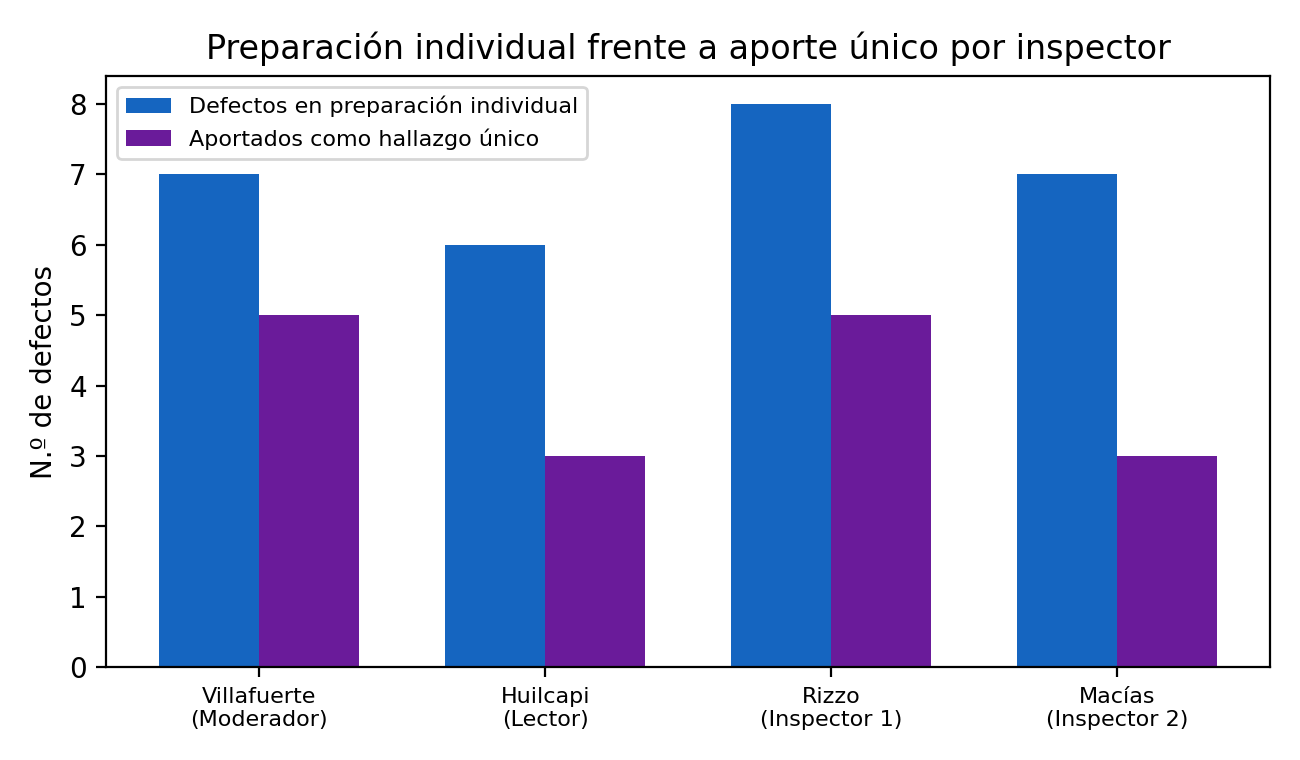
\includegraphics[width=0.72\linewidth]{figures/tasa_deteccion_inspector.png}
\caption{Defectos reportados en preparación individual y defectos aportados como hallazgo único
por cada inspector.}
\label{fig:prep}
\end{figure}

\subsection{Reunión de inspección y registro consolidado}

La reunión se realizó en 85 minutos (dentro del máximo de 90 establecido en la guía). La Lectora
parafraseó sección por sección; los inspectores reportaron sus defectos de preparación; el
Moderador consolidó las coincidencias y eliminó duplicados. Conforme a la regla de la técnica, no
se discutieron soluciones durante la reunión: toda propuesta de corrección se difirió a la
sección~5. El registro consolidado (Anexo B, reproducido aquí en su totalidad) contiene 16
defectos únicos, de los cuales 3 son críticos y 8 mayores, por encima de los mínimos exigidos
(15 defectos, al menos 3 críticos o mayores).

\begin{longtable}{p{0.9cm}p{1.6cm}p{6.3cm}p{1.9cm}p{1.4cm}p{2.4cm}}
\toprule
\textbf{N.\textordmasculine} & \textbf{Sección} & \textbf{Descripción del defecto} & \textbf{Tipo} & \textbf{Sev.} & \textbf{Req. afectado} \\
\midrule
\endfirsthead
\toprule
\textbf{N.\textordmasculine} & \textbf{Sección} & \textbf{Descripción del defecto} & \textbf{Tipo} & \textbf{Sev.} & \textbf{Req. afectado} \\
\midrule
\endhead
D-01 & \S3.2.6 & El criterio de verificación de RF-23 no especifica qué rol resuelve una inconsistencia entre peso bruto, tara y neto: solo dice que el sistema ``rechaza el registro''. & Ambigüedad & Mayor & RF-23 \\
D-02 & \S3.2.2 & RF-38 excluye la labor no presupuestada del cumplimiento del plan, pero no aclara si esa exclusión se recalcula cuando RF-27 arrastra un remanente que luego se ejecuta como labor no presupuestada. & Consistencia & Mayor & RF-27, RF-38 \\
D-03 & \S3.3 & RNF-08 exige tasa de éxito $\geq$90\,\% en personas ``sin experiencia previa'', sin excluir ni contemplar perfiles con limitación visual o auditiva en la prueba de usabilidad. & Completitud & Menor & RNF-08 \\
D-04 & \S3.2.5 & El criterio de verificación de RF-08 no define el comportamiento esperado cuando la imagen evidencia más de una deficiencia nutricional simultánea. & Verificabilidad & Mayor & RF-08 \\
D-05 & \S5.4.2 & Seis requisitos funcionales (RF-11, RF-23, RF-25, RF-32, RF-33, RF-34) dependen de una única evidencia sin plan explícito de triangulación para la Entrega 4. & Trazabilidad & Crítico & RF-11, RF-23, RF-25, RF-32, RF-33, RF-34 \\
D-06 & \S3.2.1 & RF-01 no especifica una política de bloqueo de cuenta tras intentos fallidos de autenticación. & Completitud & Mayor & RF-01 \\
D-07 & \S3.5 & RD-05 exige respaldo centralizado en la nube para la inferencia de IA, mientras que RD-02 exige operación 100\,\% funcional sin conexión; el documento no declara un modo de degradación explícito cuando el servicio de IA es inalcanzable por un período prolongado. & Consistencia & Crítico & RD-02, RD-05 \\
D-08 & \S3.2.3 & RF-15 condiciona la visualización de recorridos a la vigencia del consentimiento (RL-03), pero no define el plazo máximo en que la revocación debe propagarse al backend. & Ambigüedad & Mayor & RF-15, RL-03 \\
D-09 & \S4.2 & El flujo alternativo B de CU-06 (clasificación de sobremadurez) no tiene historia de usuario ni criterio de aceptación asociado en la Tabla~65 del ERS base. & Trazabilidad & Mayor & CU-06 \\
D-10 & \S3.2.2 & RF-36 no define el criterio de desempate cuando dos tarifas de una misma labor tienen vigencias traslapadas. & Completitud & Menor & RF-36 \\
D-11 & \S6.1 y \S5.3.3 & El cálculo WSJF identifica a RF-10 como prerrequisito técnico de RF-21, pero el MVP declara RF-10 ``No implementado'' sin registrar el riesgo de bloqueo en cadena que ello implica para la Entrega 4. & Factibilidad & Mayor & RF-10, RF-21 \\
D-12 & \S3.3 & RNF-11 exige sincronización sin pérdida ni duplicación, pero no especifica la política de resolución cuando dos dispositivos sincronizan de forma concurrente el mismo registro de avance (RF-28) tras un registro delegado. & Verificabilidad & Crítico & RNF-11, RF-28 \\
D-13 & \S3.2.7 & RF-32 declara la exclusión de datos personales en la exportación, pero no define un mecanismo de auditoría que verifique el filtro antes del envío. & Verificabilidad & Menor & RF-32 \\
D-14 & \S2.4 y \S3.4 & Agrocalidad figura en el mapa de partes interesadas con poder alto, pero ninguna fila de la Tabla~51 (requisitos legales) la traza a un RL específico. & Trazabilidad & Menor & Tabla 51 (RL) \\
D-15 & \S3.2.4 & RF-14 asume una jornada continua de rastreo GPS; no se especifica el comportamiento del conteo cuando la sesión se interrumpe a mitad de jornada por agotamiento de batería del dispositivo. & Completitud & Mayor & RF-14 \\
D-16 & \S7.3 & La limitación L-09 (conflicto de interés por consanguinidad) se declara sin fecha límite ni responsable de su resolución o cierre definitivo. & Factibilidad & Menor & L-09 \\
\bottomrule
\caption{Registro consolidado de defectos de la inspección Fagan sobre el ERS SIMPA v3.0.}
\label{tab:defectos}
\end{longtable}

\subsection{Métricas de inspección}

\begin{figure}[h]
\centering
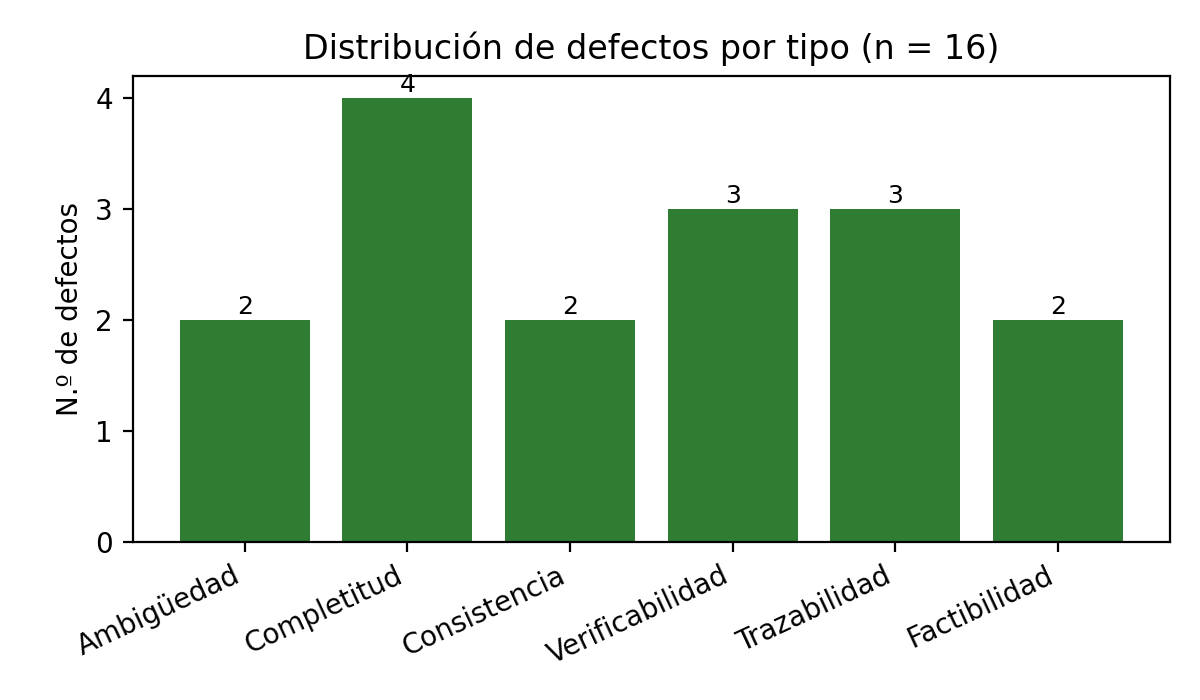
\includegraphics[width=0.62\linewidth]{figures/defectos_por_tipo.png}
\caption{Distribución de los 16 defectos consolidados por tipo (ISO/IEC/IEEE 29148:2018, \S6.4).}
\label{fig:tipo}
\end{figure}

\begin{figure}[h]
\centering
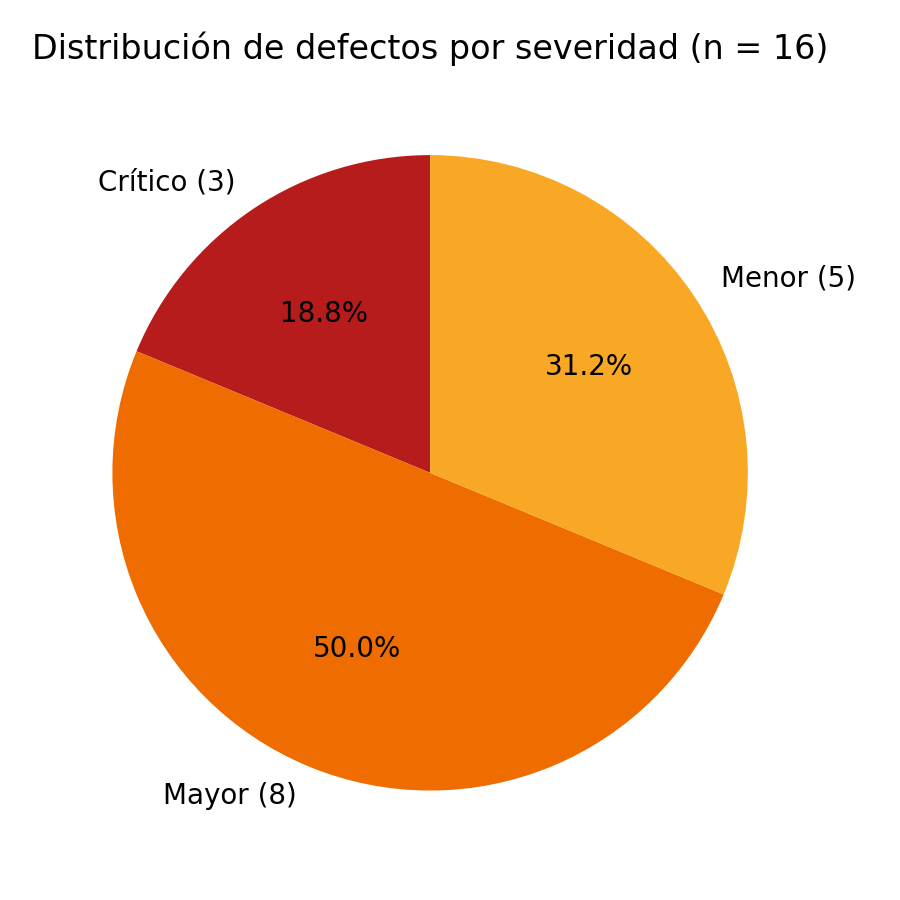
\includegraphics[width=0.55\linewidth]{figures/defectos_por_severidad.png}
\caption{Distribución de los 16 defectos consolidados por severidad.}
\label{fig:severidad}
\end{figure}

\begin{longtable}{p{2.6cm}p{3.4cm}p{8.2cm}}
\toprule
\textbf{Métrica} & \textbf{Valor} & \textbf{Interpretación} \\
\midrule
\endhead
Densidad de defectos & 16 / 40 = 0,40 def./pág. & Densidad moderada-alta para un documento en su tercera entrega; sugiere que la revisión docente previa no agotó los defectos de fondo, particularmente los de consistencia entre restricciones. \\
Tipo dominante & Completitud (4 de 16) & La mayoría de los defectos son omisiones puntuales de caso borde (baterías, tarifas traslapadas, perfiles sensoriales), no errores estructurales del documento. \\
Severidad crítica & 3 / 16 (18,8\,\%) & Los tres críticos comparten un patrón: relaciones entre requisitos (RD--RD, RNF--RF) no resueltas explícitamente, más que errores locales de redacción. \\
Redundancia entre inspectores & 28 reportes individuales $\to$ 16 únicos (42,9\,\% de solapamiento) & Indica cobertura adecuada del alcance sin exceso de redundancia que sugiera falta de independencia real entre los cuatro inspectores. \\
Esfuerzo total & 10,5 horas-persona & Costo contenido frente al beneficio: cada defecto crítico corregido aquí evita una revisión de arquitectura mucho más costosa en la Entrega 4. \\
\bottomrule
\caption{Métricas de la inspección Fagan e interpretación.}
\end{longtable}

% ============================================================
% 5. CORRECCIONES APLICADAS
% ============================================================
\section{Correcciones aplicadas}

Se corrigió el 100\,\% de los defectos críticos y mayores (11 de 16). Los cinco defectos menores
restantes se documentan como pendientes justificados: no comprometen la validez funcional del ERS
y se programan para la Entrega 4 (2B).

\begin{longtable}{p{0.7cm}p{5.3cm}p{5.3cm}p{1.5cm}}
\toprule
\textbf{ID} & \textbf{Antes} & \textbf{Después} & \textbf{Req.} \\
\midrule
\endfirsthead
\toprule
\textbf{ID} & \textbf{Antes} & \textbf{Después} & \textbf{Req.} \\
\midrule
\endhead
D-01 & ``\dots\ el sistema rechaza el registro e indica la inconsistencia.'' & ``\dots\ el sistema rechaza el registro, lo marca en estado \emph{observado} y notifica a la persona administradora para su resolución antes de reintentar el registro.'' & RF-23 \\
D-02 & Sin regla de recálculo entre RF-27 y RF-38. & Se añade postcondición a RF-27: ``Si el remanente arrastrado se ejecuta posteriormente como labor no presupuestada (RF-38), el sistema conserva su vínculo con la meta original únicamente a efectos de reporte, sin computarlo en el porcentaje de cumplimiento.'' & RF-27, RF-38 \\
D-04 & Sin caso de imagen con múltiples deficiencias. & Se añade excepción E3 a CU-02: ``Si el modelo detecta más de una deficiencia con confianza comparable, el sistema presenta ambas ordenadas por confianza y solicita a la persona usuaria priorizar la corrección.'' & RF-08, CU-02 \\
D-05 & Sin plan de triangulación declarado. & Se incorpora al plan de trabajo pendiente (\S7.5 del ERS) la actividad: ``Obtener una segunda fuente independiente para RF-11, RF-23, RF-25, RF-32, RF-33 y RF-34 antes del cierre de la Entrega 4.'' & RF-11, RF-23, RF-25, RF-32, RF-33, RF-34 \\
D-06 & Sin política de bloqueo. & Se añade a RF-01: ``Tras cinco intentos fallidos consecutivos, el sistema bloquea la cuenta por 15 minutos y registra el evento en bitácora de seguridad (RNF-13).'' & RF-01 \\
D-07 & RD-02 y RD-05 sin mecanismo de conciliación. & Se crea RF-40 mediante RFC-01 (\S6.1) como modo de operación degradada; RD-05 se reformula: ``\dots\ requiere conectividad para inferencia en línea; ante indisponibilidad prolongada, el cliente opera con los últimos umbrales sincronizados (RF-40).'' & RD-02, RD-05, RF-40 \\
D-08 & Sin plazo de propagación de revocación. & Se añade a RL-03: ``La revocación del consentimiento de geolocalización se propaga al backend en un plazo máximo de 60 segundos desde su registro en el dispositivo.'' & RF-15, RL-03 \\
D-09 & CU-06 flujo B sin HU/CA. & Se añade HU-20 / CA-20: ``Como técnico de la extractora, quiero que el sistema advierta sobremadurez, para anticipar el incremento de acidez del aceite.'' & CU-06 \\
D-11 & Riesgo de bloqueo no documentado. & Se añade a \S6.3 del ERS (desviación D-04 del prototipo): ``RF-10 se declara bloqueante de RF-21 en el plan de incorporación de la Entrega 4; ambos se implementan en el mismo incremento.'' & RF-10, RF-21 \\
D-12 & RNF-11 sin política de concurrencia. & Se reformula RNF-11 mediante RFC-02 (\S6.2): se añade política \emph{last-write-wins} con bitácora de conflicto y notificación al supervisor que efectuó el registro delegado. & RNF-11, RF-28 \\
D-15 & RF-14 sin manejo de interrupción por batería. & Se añade excepción E3 a CU-03: ``Si el dispositivo se apaga antes del cierre de jornada, el sistema conserva las marcaciones ya sincronizadas y solicita confirmar manualmente el tramo no registrado en el siguiente inicio de sesión.'' & RF-14, CU-03 \\
\bottomrule
\caption{Correcciones aplicadas a los 11 defectos críticos y mayores (antes/después).}
\label{tab:correcciones}
\end{longtable}

\noindent\textbf{Defectos menores pendientes, justificados.} D-03 (perfiles con limitación
sensorial en la prueba de RNF-08), D-10 (desempate de tarifas traslapadas), D-13 (auditoría del
filtro de exportación) y D-14 (traza de Agrocalidad a un RL) se difieren a la Entrega 4 porque su
corrección requiere una decisión de negocio (política de tarifas, alcance del módulo de
auditoría) que excede el margen de esta práctica y no compromete la operación del MVP declarada
en \S6 del ERS. D-16 se resuelve administrativamente: se fija como responsable al analista líder
y como plazo el cierre de la Entrega 4 (2B).

% ============================================================
% 6. GESTIÓN DEL CAMBIO Y CCB
% ============================================================
\section{Gestión del cambio y Change Control Board}

Se tramitaron tres RFC de naturaleza distinta. RFC-01 nace directamente del defecto crítico D-07
detectado en la inspección; RFC-02 nace del defecto crítico D-12; RFC-03 responde a un escenario
normativo publicado por la cátedra sobre el plazo de retención de datos de geolocalización
laboral, no derivado de la inspección.

\subsection{RFC-01 --- Alcance: modo de operación degradada del componente de IA}

\begin{longtable}{p{3cm}p{10.8cm}}
\toprule
\textbf{Campo} & \textbf{Contenido} \\
\midrule
\endhead
ID / Fecha / Solicitante & RFC-01 / 04-08-2026 / Villafuerte Rosero Allan Noe (analista líder) \\
Requisito afectado & RD-02, RD-05 \\
Descripción & Incorporar el requisito funcional RF-40: ``Modo de operación degradada sin inferencia remota'', que permite al cliente móvil operar con los últimos umbrales de variedad y de madurez sincronizados cuando el servicio de IA es inalcanzable por más de 4 horas continuas. \\
Justificación de negocio & Sin este mecanismo, RD-02 (operación 100\,\% offline) y RD-05 (inferencia centralizada en la nube) son mutuamente incompatibles en la práctica: el 74,2\,\% del personal no tiene conectividad permanente (EV-12), por lo que la ausencia de un modo degradado deja sin diagnóstico útil a la mayoría de las jornadas de campo. \\
Requisitos impactados (matriz) & Directos: RD-02, RD-05, RNF-04, RNF-11, RNF-17. Indirectos (vía CU-01, CU-02, CU-06, que incluyen obligatoriamente a CU-18): RF-07, RF-08, RF-21, RNF-16. \\
Artefactos impactados & CU-01, CU-02, CU-06; clase \texttt{Variedad} y \texttt{Diagnostico} del diagrama de clases; mockup MU-03; componente ``Orquestador de IA'' del diagrama de componentes. \\
Costo estimado & 21 horas-persona (cach\'e local de umbrales, lógica de expiración de 4 horas, indicador visual de resultado ``no verificado en línea''). \\
Riesgo & Un diagnóstico con umbrales desactualizados podría inducir a error si la variedad del lote cambia entre sincronizaciones; se mitiga marcando todo resultado degradado como ``no verificado'' en la interfaz. \\
Recomendación técnica & Aprobar; el costo es bajo frente al riesgo de que el 74,2\,\% del personal quede sin la función mejor valorada del cuestionario (RF-07, 4,27/5). \\
\bottomrule
\caption{RFC-01 -- Modo de operación degradada.}
\end{longtable}

\subsection{RFC-02 --- Calidad: política de concurrencia de RNF-11}

\begin{longtable}{p{3cm}p{10.8cm}}
\toprule
\textbf{Campo} & \textbf{Contenido} \\
\midrule
\endhead
ID / Fecha / Solicitante & RFC-02 / 04-08-2026 / Rizzo Vélez Edson Nagib (verificador) \\
Requisito afectado & RNF-11 \\
Descripción & Modificar RNF-11 para incorporar una política explícita de resolución de conflictos de sincronización concurrente: \emph{last-write-wins} sobre el campo \texttt{fechaRegistro}, con bitácora de conflicto accesible al supervisor que efectuó el registro delegado (RF-35). \\
Justificación de negocio & El registro delegado (RF-35) habilita a un supervisor a registrar en nombre de un trabajador sin dispositivo propio; si ese mismo trabajador consigue luego un dispositivo prestado y registra el mismo avance, RNF-11 no define cuál de los dos registros prevalece, arriesgando una duplicación silenciosa del pago por avance. \\
Requisitos impactados (matriz) & Directos: RNF-11, RF-28, RF-35. Indirectos: RF-29 (cálculo de remuneración), RF-37 (liquidación semanal). \\
Artefactos impactados & CU-04 (flujo alternativo A, registro delegado); clase \texttt{RegistroAvance}; componente ``Motor de sincronización''. \\
Costo estimado & 13 horas-persona. \\
Riesgo & Bajo; la política \emph{last-write-wins} es estándar en sistemas \emph{offline-first} y no introduce dependencia nueva. \\
Recomendación técnica & Aprobar sin condiciones. \\
\bottomrule
\caption{RFC-02 -- Política de concurrencia de sincronización.}
\end{longtable}

\subsection{RFC-03 --- Restricción/normativa: plazo de retención de datos de geolocalización}

\begin{longtable}{p{3cm}p{10.8cm}}
\toprule
\textbf{Campo} & \textbf{Contenido} \\
\midrule
\endhead
ID / Fecha / Solicitante & RFC-03 / 04-08-2026 / Alcívar Vélez Anderson Adonis (apoyo repositorio), a partir del escenario normativo n.\textordmasculine\ 2 publicado en el SGA sobre plazos de retención de datos laborales de geolocalización. \\
Requisito afectado & RL-06, RNF-14 \\
Descripción & Incorporar la restricción RD-11: ``Los datos de geolocalización individual (marcaciones GPS, recorridos) se purgan automáticamente a los 12 meses de su captura, conservando únicamente los agregados no identificables usados en RF-16 (evaluación de desempeño).'' \\
Justificación de negocio & El principio de minimización de la LOPDP (Art.~10, ya trazado en RL-02) exige limitar tanto el alcance como la duración del tratamiento; el ERS v3.0 no fija un plazo de retención para los datos de geolocalización, lo que constituye un vacío frente al escenario normativo evaluado por la cátedra. \\
Requisitos impactados (matriz) & Directos: RL-06, RNF-14, RD-11 (nuevo). Indirectos: RF-15, RF-14, RF-16. \\
Artefactos impactados & Componente ``Bitácora de acceso''; clase \texttt{Marcacion} y \texttt{Recorrido}; tarea programada de purga en el backend (nuevo componente no modelado previamente). \\
Costo estimado & 8 horas-persona. \\
Riesgo & Si la purga elimina datos necesarios para una auditoría de calidad en curso (RF-24), podría perderse evidencia; se mitiga excluyendo de la purga los recorridos vinculados a una calificación desfavorable de la extractora hasta el cierre de esa auditoría. \\
Recomendación técnica & Aprobar; es de cumplimiento obligatorio y de costo bajo. \\
\bottomrule
\caption{RFC-03 -- Plazo de retención de datos de geolocalización.}
\end{longtable}

\subsection{Acta del Change Control Board}

\noindent\textbf{Fecha:} 04 de agosto de 2026. \textbf{Asistentes:} Villafuerte Rosero Allan Noe
(Presidente), Arboleda Yanza Francisco Javier (Representante del cliente, en simulación del rol
de Administrador general), Huilcapi León Denisses Fabiola (Analista), Rizzo Vélez Edson Nagib
(Desarrollador), Macías Herrera Josthyn Esteban (Secretario, redacción del acta), Alcívar Vélez
Anderson Adonis (Verificador de la matriz de trazabilidad durante la sesión).

\noindent\textbf{Agenda:} (1) presentación de RFC-01 a RFC-03 por su solicitante; (2)
deliberación; (3) votación; (4) definición de responsables y plazos; (5) cierre de versión.

\begin{longtable}{p{1.6cm}p{5.7cm}p{2.4cm}p{4cm}}
\toprule
\textbf{RFC} & \textbf{Deliberación resumida} & \textbf{Decisión} & \textbf{Responsable / plazo} \\
\midrule
\endhead
RFC-01 & El representante del cliente valora la mejora pero advierte que el modo degradado no debe implementarse en el MVP actual (5.\S6.1 del ERS), dado que el prototipo aún no integra inferencia real. El desarrollador confirma que el costo (21 h-p) es asumible en la Entrega 4. & \textbf{Aprobado con condiciones}: se incorpora al ERS y a la matriz de trazabilidad, pero su implementación se programa para la Entrega 4, no para el MVP vigente. & Rizzo Vélez (desarrollador) / cierre de Entrega 4 (2B) \\
RFC-02 & Sin objeciones; el analista señala que la política \emph{last-write-wins} es coherente con el patrón ya usado en RF-04 (flujo alternativo B, sin conectividad). & \textbf{Aprobado} & Rizzo Vélez (desarrollador) / próxima iteración de \texttt{RegistroAvance} \\
RFC-03 & El representante del cliente confirma que la organización no ha definido internamente un plazo de retención; el analista recuerda que RL-06 (derecho de eliminación) ya obliga a un mecanismo de purga, por lo que RD-11 lo hace explícito y automático. & \textbf{Aprobado} & Alcívar Vélez (repositorio) y Huilcapi León (documentación) / incorporación inmediata al ERS \\
\bottomrule
\caption{Acta resumida del Change Control Board del 04-08-2026.}
\end{longtable}

\noindent\textbf{Versión resultante.} Las tres RFC aprobadas se incorporan en una nueva versión
del ERS, \textbf{v3.1}, publicada como línea base \texttt{baseline-v3.1} (\S8). El historial de
revisiones del documento se actualiza con la entrada correspondiente en el
\texttt{CHANGELOG.md} del repositorio (Anexo E).

\noindent\textbf{Firman:} Villafuerte Rosero A.\ N., Huilcapi León D.\ F., Rizzo Vélez E.\ N.,
Macías Herrera J.\ E., Arboleda Yanza F.\ J., Alcívar Vélez A.\ A.

% ============================================================
% 7. TRAZABILIDAD EN HERRAMIENTA CASE
% ============================================================
\section{Trazabilidad en herramienta CASE}

Se construyó el tablero \textbf{Jira} del proyecto \texttt{SIMPA} (clave de proyecto
\texttt{SIM}), con acceso otorgado a los seis integrantes y al docente.

\subsection{Estructura del backlog}

\begin{center}
\begin{tabular}{p{3.2cm}p{9.5cm}}
\toprule
\textbf{Epic} & \textbf{Alcance} \\
\midrule
SIM-E1 Estructura productiva & RF-01 a RF-03, RF-10 (autenticación, lotes, personal, variedades) \\
SIM-E2 Planificación y labores & RF-04, RF-26 a RF-29, RF-35 a RF-39 \\
SIM-E3 Diagnóstico asistido por IA & RF-05, RF-07 a RF-09, RF-12, RF-21, RF-22, RF-40 (RFC-01) \\
SIM-E4 Calidad y relación con la extractora & RF-23 a RF-25, RF-30 a RF-33 \\
SIM-E5 Reportes y trazabilidad histórica & RF-06, RF-11, RF-13 a RF-20 \\
\bottomrule
\end{tabular}
\end{center}

\noindent Bajo las cinco épicas se crearon 20 \emph{Stories}, una por requisito funcional Must o
Should representativo (RF-01, RF-02, RF-04, RF-05, RF-07, RF-08, RF-10, RF-12, RF-13, RF-14,
RF-15, RF-19, RF-21, RF-22, RF-23, RF-26, RF-28, RF-30, RF-35, RF-40), superando el mínimo de 15.
Se agregaron \emph{Sub-tasks} de criterio de aceptación (mínimo 2 cada una) para cinco historias:
SIM-4 (RF-04 / HU-04), SIM-7 (RF-07 / HU-06), SIM-11 (RF-14 / HU-11), SIM-16 (RF-26 / HU-16) y
SIM-19 (RF-35 / HU-19).

\subsection{Campos personalizados}

\begin{center}
\begin{tabular}{lll}
\toprule
\textbf{Campo} & \textbf{Tipo} & \textbf{Ejemplo} \\
\midrule
Prioridad MoSCoW & Lista desplegable & Must / Should / Could \\
Fuente del requisito & Texto corto (ID de evidencia) & EV-01, EV-12, EV-13 \\
Estado de verificación & Lista desplegable (campo adicional valorado) & Pendiente / Verificado en inspección / Corregido \\
\bottomrule
\end{tabular}
\end{center}

\subsection{Trazabilidad bidireccional y evidencias}

Cada \emph{Story} enlaza hacia atrás, mediante el campo ``Fuente del requisito'' y una etiqueta
\texttt{stakeholder:*}, al participante o documento de origen (por ejemplo,
\texttt{stakeholder:ENTR-04} para RF-21); y hacia adelante, mediante enlaces \emph{relates to} /
\emph{is tested by}, al caso de uso, la clase del diagrama y el caso de prueba correspondientes.
Los tres requisitos que la inspección marcó como huérfanos de artefacto (RF-03, RF-27, RF-34, sin
mockup en el ERS base) se reportan explícitamente en el tablero con la etiqueta
\texttt{sin-mockup} en lugar de omitirse.

\noindent\textbf{Evidencias.} Se referencian en el repositorio, dentro de
\texttt{04\_Trazabilidad/capturas/}: captura del tablero completo
(\texttt{tablero\_completo.png}), detalle de tres issues con sus enlaces visibles
(\texttt{SIM-7\_detalle.png}, \texttt{SIM-14\_detalle.png}, \texttt{SIM-19\_detalle.png}) y panel
de estadísticas (\texttt{panel\_estadisticas.png}). \emph{El equipo debe sustituir estos
marcadores por sus capturas reales del tablero antes de la entrega final}, conforme al criterio
de admisión A2 de la guía. La exportación a CSV del backlog se referencia como
\texttt{04\_Trazabilidad/backlog\_export.csv} (Anexo D).

\subsection{Matriz de trazabilidad (vista de 16 filas)}

\begin{longtable}{p{2.6cm}p{1.1cm}p{1.1cm}p{3.4cm}p{3.6cm}}
\toprule
\textbf{Stakeholder} & \textbf{RF} & \textbf{CU} & \textbf{Clase / Módulo} & \textbf{Prueba} \\
\midrule
\endhead
Administrador general (EV-01) & RF-01 & CU-11 & \texttt{Usuario.autenticar()} & PT-01 Bloqueo tras 5 intentos (D-06) \\
Administrador general (EV-01) & RF-02 & CU-12 & \texttt{Lote} & PT-02 Alta de lote y selección en labor \\
Asistente admin. (EV-07) & RF-04 & CU-04 & \texttt{Labor}, \texttt{RegistroAvance} & PT-03 Registro sin conexión (RNF-11) \\
Trabajador agrícola (EV-05) & RF-05 & CU-15 & \texttt{Palma.marcarAfectada()} & PT-04 Filtro de incidencia abierta \\
Asistente admin. (EV-07) & RF-07 & CU-01 & Orquestador de IA / \texttt{DiagnosticoPlaga} & PT-05 Confianza insuficiente (flujo B) \\
Asesor técnico (EV-02) & RF-08 & CU-02 & \texttt{DiagnosticoNutricional} & PT-06 Múltiples deficiencias (D-04) \\
Asesor técnico (EV-04) & RF-10 & CU-12 & \texttt{Variedad} & PT-07 Umbral por variedad \\
Administrador general (EV-01) & RF-12 & CU-16 & \texttt{Alerta} & PT-08 Alerta ante diagnóstico positivo \\
Jefe polinización (EV-03) & RF-13 & CU-03 & \texttt{RegistroPolinizacion} & PT-09 Estado de antesis \\
Jefe polinización (EV-03) & RF-14 & CU-03 & \texttt{Marcacion.esPrecisa()} & PT-10 Interrupción por batería (D-15) \\
Administrador general (EV-01) & RF-15 & CU-03 & \texttt{Recorrido} & PT-11 Consentimiento revocado (D-08) \\
Administrador general (EV-11) & RF-19 & CU-05 & \texttt{Reporte} & PT-12 Consolidado semanal exportable \\
Téc. extractora (EV-04) & RF-21 & CU-06 & \texttt{ClasificacionMadurez.clasificar()} & PT-13 Umbral guineensis vs.\ híbrido \\
Administrador (EV-04, EV-08) & RF-22 & CU-06 & \texttt{Lote.porcentajeFrutaVerde()} & PT-14 Alerta preventiva de despacho \\
Téc. extractora (EV-04) & RF-23 & CU-10 & \texttt{CalificacionExtractora} & PT-15 Inconsistencia bruto-tara-neto (D-01) \\
Jefe de campo (EV-12) & RF-35 & CU-04 & \texttt{Labor.registroDelegado} & PT-16 Concurrencia de sincronización (D-12) \\
\bottomrule
\caption{Matriz de trazabilidad extendida (16 filas, coherente con el tablero Jira).}
\label{tab:matriz-case}
\end{longtable}



\end{document}
